% Template for a Computer Science Tripos Part II project dissertation
\documentclass[12pt,a4paper,twoside,openright]{report}
\usepackage[pdfborder={0 0 0}]{hyperref}    % turns references into hyperlinks
\usepackage[margin=25mm]{geometry}  % adjusts page layout
\usepackage{graphicx}  % allows inclusion of PDF, PNG and JPG images
\usepackage{verbatim}
\usepackage{docmute}   % only needed to allow inclusion of proposal.tex

\raggedbottom                           % try to avoid widows and orphans
\sloppy
\clubpenalty1000%
\widowpenalty1000%

\renewcommand{\baselinestretch}{1.1}    % adjust line spacing to make
                                        % more readable

\begin{document}

\bibliographystyle{plain}


%%%%%%%%%%%%%%%%%%%%%%%%%%%%%%%%%%%%%%%%%%%%%%%%%%%%%%%%%%%%%%%%%%%%%%%%
% Title


\pagestyle{empty}

\rightline{\LARGE \textbf{Martin Richards}}

\vspace*{60mm}
\begin{center}
\Huge
\textbf{How to write a dissertation in \LaTeX} \\[5mm]
Computer Science Tripos -- Part II \\[5mm]
St John's College \\[5mm]
\today  % today's date
\end{center}

%%%%%%%%%%%%%%%%%%%%%%%%%%%%%%%%%%%%%%%%%%%%%%%%%%%%%%%%%%%%%%%%%%%%%%%%%%%%%%
% Proforma, table of contents and list of figures

\pagestyle{plain}

\chapter*{Proforma}

{\large
\begin{tabular}{ll}
Name:               & \bf Martin Richards                       \\
College:            & \bf St John's College                     \\
Project Title:      & \bf How to write a dissertation in \LaTeX \\
Examination:        & \bf Computer Science Tripos -- Part II, July 2001  \\
Word Count:         & \bf 1587\footnotemark[1]
                      (well less than the 12000 limit)  \\
Project Originator: & Dr M.~Richards                    \\
Supervisor:         & Dr Markus Kuhn                    \\ 
\end{tabular}
}
\footnotetext[1]{This word count was computed
by \texttt{detex diss.tex | tr -cd '0-9A-Za-z $\tt\backslash$n' | wc -w}
}
\stepcounter{footnote}


\section*{Original Aims of the Project}

To write a demonstration dissertation\footnote{A normal footnote without the
complication of being in a table.} using \LaTeX\ to save
student's time when writing their own dissertations. The dissertation
should illustrate how to use the more common \LaTeX\ constructs. It
should include pictures and diagrams to show how these can be
incorporated into the dissertation.  It should contain the entire
\LaTeX\ source of the dissertation and the makefile.  It should
explain how to construct an MSDOS disk of the dissertation in
Postscript format that can be used by the book shop for printing, and,
finally, it should have the prescribed layout and format of a diploma
dissertation.


\section*{Work Completed}

All that has been completed appears in this dissertation.

\section*{Special Difficulties}

Learning how to incorporate encapulated postscript into a \LaTeX\
document on both Ubuntu Linux and OS X.
 
\newpage
\section*{Declaration}

I, [Name] of [College], being a candidate for Part II of the Computer
Science Tripos [or the Diploma in Computer Science], hereby declare
that this dissertation and the work described in it are my own work,
unaided except as may be specified below, and that the dissertation
does not contain material that has already been used to any substantial
extent for a comparable purpose.

\bigskip
\leftline{Signed [signature]}

\medskip
\leftline{Date [date]}

\tableofcontents

\listoffigures

\newpage
\section*{Acknowledgements}

This document owes much to an earlier version written by Simon Moore
\cite{Moore95}.  His help, encouragement and advice was greatly 
appreciated.

%%%%%%%%%%%%%%%%%%%%%%%%%%%%%%%%%%%%%%%%%%%%%%%%%%%%%%%%%%%%%%%%%%%%%%%
% now for the chapters

\pagestyle{headings}

\chapter{Introduction}

\section{Overview of the files}

This document consists of the following files:

\begin{itemize}
\item \texttt{makefile} --- The makefile for the dissertation and
                         Project Proposal
\item \texttt{diss.tex} --- The dissertation
\item \texttt{proposal.tex}  --- The project proposal 
\item \texttt{figs} -- A directory containing diagrams and pictures
\item \texttt{refs.bib} --- The bibliography database
\end{itemize}

\section{Building the document}

This document was produced using \LaTeXe which is based upon
\LaTeX\cite{Lamport86}.  To build the document you first need to
generate \texttt{diss.aux} which, amongst other things, contains the
references used.  This if done by executing the command:

\texttt{pdflatex diss}

\noindent
Then the bibliography can be generated from \texttt{refs.bib} using:

\texttt{bibtex diss}

\noindent
Finally, to ensure all the page numbering is correct run \texttt{pdflatex}
on \texttt{diss.tex} until the \texttt{.aux} files do not change.  This
usually takes 2 more runs.

\subsection{The makefile}

To simplify the calls to \texttt{pdflatex} and \texttt{bibtex}, 
a makefile has been provided, see Appendix~\ref{makefile}. 
It provides the following facilities:

\begin{description}

\item\texttt{make} \\
 Display help information.

\item\texttt{make proposal.pdf} \\
 Format the proposal document as a PDF.

\item\texttt{make view-proposal} \\
 Run \texttt{make proposal.pdf} and then display it with a Linux PDF viewer
 (preferably ``okular'', if that is not available fall back to ``evince'').

\item\texttt{make diss.pdf} \\
 Format the dissertation document as a PDF.

\item\texttt{make count} \\
Display an estimate of the word count.

\item\texttt{make all} \\
Construct \texttt{proposal.pdf} and \texttt{diss.pdf}.

\item\texttt{make pub} \\ Make \texttt{diss.pdf}
and place it in my \texttt{public\_html} directory.

\item\texttt{make clean} \\ Delete all intermediate files except the
source files and the resulting PDFs. All these deleted files can
be reconstructed by typing \texttt{make all}.

\end{description}


\section{Counting words}

An approximate word count of the body of the dissertation may be
obtained using:

\texttt{wc diss.tex}

\noindent
Alternatively, try something like:

\verb/detex diss.tex | tr -cd '0-9A-Z a-z\n' | wc -w/


\chapter{Preparation}

This chapter is empty!


\chapter{Implementation}

\section{Verbatim text}

Verbatim text can be included using \verb|\begin{verbatim}| and
\verb|\end{verbatim}|. I normally use a slightly smaller font and
often squeeze the lines a little closer together, as in:

{\renewcommand{\baselinestretch}{0.8}\small
\begin{verbatim}
GET "libhdr"
 
GLOBAL { count:200; all  }
 
LET try(ld, row, rd) BE TEST row=all
                        THEN count := count + 1
                        ELSE { LET poss = all & ~(ld | row | rd)
                               UNTIL poss=0 DO
                               { LET p = poss & -poss
                                 poss := poss - p
                                 try(ld+p << 1, row+p, rd+p >> 1)
                               }
                             }
LET start() = VALOF
{ all := 1
  FOR i = 1 TO 12 DO
  { count := 0
    try(0, 0, 0)
    writef("Number of solutions to %i2-queens is %i5*n", i, count)
    all := 2*all + 1
  }
  RESULTIS 0
}
\end{verbatim}
}

\section{Tables}

\begin{samepage}
Here is a simple example\footnote{A footnote} of a table.

\begin{center}
\begin{tabular}{l|c|r}
Left      & Centred & Right \\
Justified &         & Justified \\[3mm]
%\hline\\%[-2mm]
First     & A       & XXX \\
Second    & AA      & XX  \\
Last      & AAA     & X   \\
\end{tabular}
\end{center}

\noindent
There is another example table in the proforma.
\end{samepage}

\section{Simple diagrams}

Simple diagrams can be written directly in \LaTeX.  For example, see
figure~\ref{latexpic1} on page~\pageref{latexpic1} and see
figure~\ref{latexpic2} on page~\pageref{latexpic2}.

\begin{figure}
\setlength{\unitlength}{1mm}
\begin{center}
\begin{picture}(125,100)
\put(0,80){\framebox(50,10){AAA}}
\put(0,60){\framebox(50,10){BBB}}
\put(0,40){\framebox(50,10){CCC}}
\put(0,20){\framebox(50,10){DDD}}
\put(0,00){\framebox(50,10){EEE}}

\put(75,80){\framebox(50,10){XXX}}
\put(75,60){\framebox(50,10){YYY}}
\put(75,40){\framebox(50,10){ZZZ}}

\put(25,80){\vector(0,-1){10}}
\put(25,60){\vector(0,-1){10}}
\put(25,50){\vector(0,1){10}}
\put(25,40){\vector(0,-1){10}}
\put(25,20){\vector(0,-1){10}}

\put(100,80){\vector(0,-1){10}}
\put(100,70){\vector(0,1){10}}
\put(100,60){\vector(0,-1){10}}
\put(100,50){\vector(0,1){10}}

\put(50,65){\vector(1,0){25}}
\put(75,65){\vector(-1,0){25}}
\end{picture}
\end{center}
\caption{A picture composed of boxes and vectors.}
\label{latexpic1}
\end{figure}

\begin{figure}
\setlength{\unitlength}{1mm}
\begin{center}

\begin{picture}(100,70)
\put(47,65){\circle{10}}
\put(45,64){abc}

\put(37,45){\circle{10}}
\put(37,51){\line(1,1){7}}
\put(35,44){def}

\put(57,25){\circle{10}}
\put(57,31){\line(-1,3){9}}
\put(57,31){\line(-3,2){15}}
\put(55,24){ghi}

\put(32,0){\framebox(10,10){A}}
\put(52,0){\framebox(10,10){B}}
\put(37,12){\line(0,1){26}}
\put(37,12){\line(2,1){15}}
\put(57,12){\line(0,2){6}}
\end{picture}

\end{center}
\caption{A diagram composed of circles, lines and boxes.}
\label{latexpic2}
\end{figure}



\section{Adding more complicated graphics}

The use of \LaTeX\ format can be tedious and it is often better to use
encapsulated postscript (EPS) or PDF to represent complicated graphics.
Figure~\ref{epsfig} and~\ref{xfig} on page \pageref{xfig} are
examples. The second figure was drawn using \texttt{xfig} and exported in
{\tt.eps} format. This is my recommended way of drawing all diagrams.


\begin{figure}[tbh]
\centerline{
\includegraphics{figs/cuarms.pdf}}
\caption{Example figure using encapsulated postscript}
\label{epsfig}
\end{figure}

\begin{figure}[tbh]
\vspace{4in}
\caption{Example figure where a picture can be pasted in}
\label{pastedfig}
\end{figure}


\begin{figure}[tbh]
\centerline{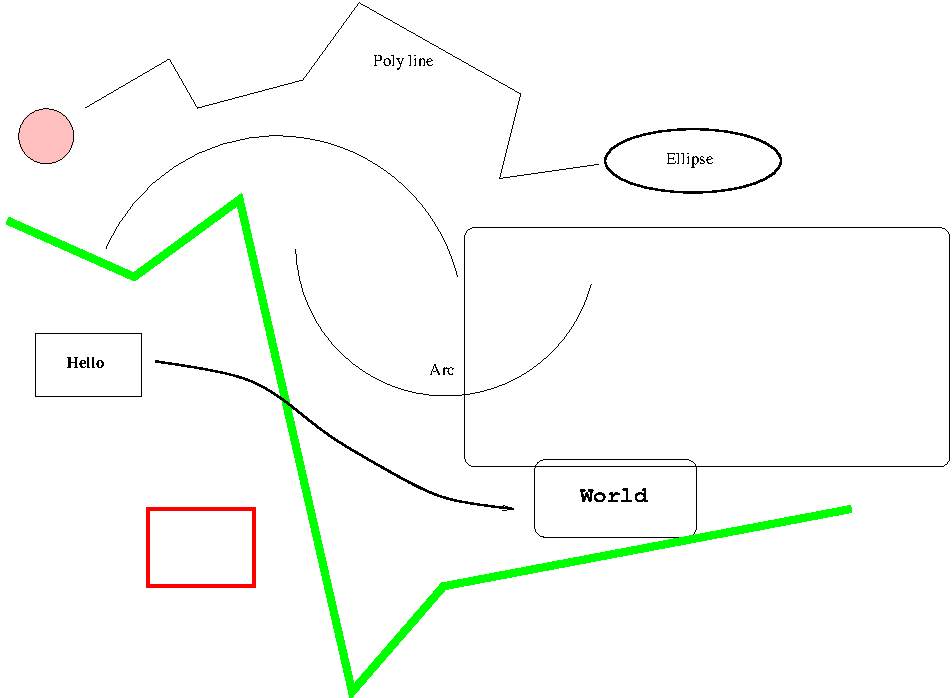
\includegraphics{figs/diagram.pdf}}
\caption{Example diagram drawn using \texttt{xfig}}
\label{xfig}
\end{figure}


\chapter{Evaluation}

\section{Printing and binding}

Use a ``duplex'' laser printer that can print on both sides to print
two copies of your dissertation. Then bind them, for example using the
comb binder in the Computer Laboratory Library.

\section{Further information}

See the Unix Tools notes at

\url{http://www.cl.cam.ac.uk/teaching/current-1/UnixTools/materials.html}


\chapter{Conclusion}

I hope that this rough guide to writing a dissertation is \LaTeX\ has
been helpful and saved you time.


%%%%%%%%%%%%%%%%%%%%%%%%%%%%%%%%%%%%%%%%%%%%%%%%%%%%%%%%%%%%%%%%%%%%%
% the bibliography
\addcontentsline{toc}{chapter}{Bibliography}
\bibliography{refs}

%%%%%%%%%%%%%%%%%%%%%%%%%%%%%%%%%%%%%%%%%%%%%%%%%%%%%%%%%%%%%%%%%%%%%
% the appendices
\appendix

\chapter{Latex source}

\section{diss.tex}
{\scriptsize\verbatiminput{diss.tex}}

\section{proposal.tex}
{\scriptsize\verbatiminput{proposal.tex}}

\chapter{Makefile}

\section{makefile}\label{makefile}
{\scriptsize\verbatiminput{makefile.txt}}

\section{refs.bib}
{\scriptsize\verbatiminput{refs.bib}}


\chapter{Project Proposal}

% Note: this file can be compiled on its own, but is also included by
% diss.tex (using the docmute.sty package to ignore the preamble)
\documentclass[12pt,a4paper,twoside]{article}
\usepackage[UKenglish]{isodate}
\usepackage[pdfborder={0 0 0}]{hyperref}
\usepackage[margin=25mm]{geometry}
\usepackage{graphicx}
\usepackage{parskip}
\usepackage{enumitem}
% \usepackage{mathpazo}
% \usepackage{eulervm}
\usepackage{microtype}

\usepackage[style=numeric,backend=bibtex]{biblatex}
\bibliography{refs.bib}

\begin{document}

\cleanlookdateon

\begin{center}
\Large
Computer Science Tripos -- Part II -- Project Proposal\\[4mm]
\LARGE
A Comparison of Statistical Models and Recurrent Neural Networks Applied to the
Generation of Music\\[4mm]

\large
Alex Coplan, St Catharine's College

Originator: Alex Coplan

\today
\end{center}

\vspace{5mm}

\textbf{Project Supervisor:} Matthew Ireland

\textbf{Director of Studies:} Dr S. Taraskin

\textbf{Project Overseers:} Dr M. Fiore \& Dr I. Leslie

% Main document

\section*{Introduction}

The goal of this project is to implement, evaluate, and compare two different
techniques for the algorithmic generation of music. I am particularly interested
in the generation of melody, and ultimately, \emph{polyphony}: multiple
independent melodies interacting with each other in harmonic coherence. In
particular, the two classes of techniques I intend to consider for this project
are:
\begin{itemize}[itemsep=0mm]
	\item Statistical history models such as \emph{multiple viewpoint
			systems} \cite{conklin1995viewpoints}.
	\item Recurrent neural networks.
\end{itemize}

The exact statistical model(s) to be investigated will be determined by the end
of the research phase of the project.

Algorithmic composition is of general interest in computational creativity, but
also has a number of practical applications; one such application being in
\emph{machine-assisted composition}, where a music generation tool aids a human
composer by extending or generating musical ideas. Such tools would be used by a
wide variety of music practitioners.

My intention is to undertake an investigation into the algorithmic composition
of polyphonic music. The first major problem that needs to be tackled in such an
endeavour is that of melody generation. Once this problem has been addressed,
one would subsequently consider the problem ``given a melody (the
\emph{subject}), compose a second (independent) melody (the
\emph{countersubject}) which interacts with, and is coherent with the subject.''
Since the lines in polyphony should be \emph{independent} melodies, it is
necessary to approach the problem of melody generation first.

I therefore propose that the core of the project investigate the application of
these techniques to melody generation. As an optional extension, an
investigation could then be carried out into the composition of two-part
polyphonic music, using these techniques and/or extensions thereof.

I shall follow the approach often taken in the literature of restricting the
domain of source material to stem from a particular musical idiom, e.g.\
\cite{pearce2001evaluation}. This is desirable for a number of reasons, not
least because it introduces a useful evaluation criterion: do the compositions
produced by the system exhibit a coherent musical style, consistent with that
exhibited by the material in the corpus?

In order for this project to be evaluated effectively, in addition to any
information-theoretic or music-theoretic analyses, it is necessary to perform
listening trials on human subjects. Pearce et al.\ \cite{pearce2001evaluation}
outline a framework for evaluation which allows more scientific claims to be
made as a result of the evaluation process. Evaluation would be performed in the
form of a blind trial where the subjects are asked to classify compositions as
human or machine-composed. In this work, it is noted that the participants
exhibited a bias towards classifying compositions as machine composed. This is
something that should be taken into account when designing the evaluation
methodology. An avenue for investigation in this respect is the method of
\emph{three-alternative forced choice}.

Conklin \cite{conklin2003music} notes that random walk is not necessarily the
best method of sampling from a statistical distribution such as that of a
multiple viewpoint system or Markov chain. In this project, I would therefore
also consider exploring different techniques for sampling from statistical
models.
 
\subsection*{Background}

Markov processes are natural statistical models for the analysis of melody, and
are well known as tools for composition \cite{ames1989markov}. Although
effective, Markov processes are far from perfect tools for modelling music.
Specifically, a basic pitch-duration Markov process disregards a considerable
amount of musical information available in the context
\cite{conklin1995viewpoints}.  

However, simply incorporating more musical features into the state space of a
Markov chain leads to an exponential blow-up in space complexity and
necessitates both a large amount of training data for good performance, as well
as solving the sparse data problem (\cite{conklin2003music}, section 2.1).
Moreover, Markov chains do not make use of the long-term context of a system,
which is necessary for modelling the broader sense of sequence and structure
which is present in music.

Conklin et al.\ \cite{conklin1995viewpoints} introduce the method of
\emph{multiple viewpoints} which uses the interpolation of the predictions of
many different context models, each of which considers a different musical
attribute (or some combination of attributes). These include both short-term and
long-term attributes, enabling this method to capture sequence and structure.

It is well known that Recurrent Neural Networks (RNNs) can effectively generate
sequences. RNNs have seen more successful application in music following the
introduction of long short-term memory (LSTM) techniques \cite{eck2002lstm}.
Without use of LSTM, RNNs exhibit similar problems to Markov chains in that the
output does not contain the elements of sequence and structure that one might
expect from compositions in the corpus.

\section*{Starting point}

In Lent term of 2016, I gave a talk (as part of Churchill college's Computer
Science talk series) on melody generation using Markov chains. I also
constructed a demo in Ruby which implemented a parser for ABC
notation\footnote{\url{http://abcnotation.com/}} along with a simple Markov
chain model, trained of a small corpus of hymn tunes, which generated tunes by
random walk. 

Although this experience led me to this choice of project, the implementation of
a model such as a multiple viewpoint system is considerably more involved, and
the architecture vastly different. The implementation of this model will
therefore be carried out from scratch.  The neural network will be implemented
using a library such as Google's
TensorFlow\footnote{\url{https://www.tensorflow.org/}}.

As an organ scholar (and previously an A-Level music student), I have
considerable experience with performing polyphonic music (and some experience of
analysis), especially that of the renaissance and baroque eras. I believe this
domain knowledge will prove especially useful for making musically-informed
decisions in this project. 

\section*{Resources required}

For this project I shall primarily use my own laptop. Backup will be primarily
in the form of a GitHub-hosted repository, but I will also perform backups of
the project files to an external hard drive as well as multiple cloud providers
(Google, Apple, Dropbox) and the MCS. Should my main computer suddenly fail, I
can easily continue the project using MCS computers by cloning the code from the
GitHub repository.

Although datasets can easily be compiled from online sources, it may also be of
use to have a MIDI keyboard to be able to input arbitrary musical data. I own a
MIDI keyboard which would be suitable for these purposes. I will make use of
open-source software (such as MuseScore\footnote{\url{https://musescore.org/}})
for synthesis of MIDI and other musical data. I require no other special
resources.

\section*{Work to be done}

I will employ an agile software development methodology when undertaking this
project. The ordered list of sub-tasks within this project are:
\begin{enumerate}

\item Devising and implementing an internal representation of musical data,
	along with a simple ``music theory engine'' to process this data.  

\item Implementing a simple parser for some form of input notation (ABC, MIDI,
	MusicXML); the exact form to be determined in the research phase.  

\item Implementing and iteratively refining the statistical model (e.g. multiple
	viewpoint system).

\item Implementing and iteratively refining the RNN for melody generation.  

\item Designing and carrying out a scheme for human evaluation.

\item Making iterative improvements to the two models.

\end{enumerate}

\section*{Success criteria}

\subsection*{Core Tasks}

The project will be a success if I have:
\begin{itemize}
	\item Successfully implemented a statistical model such as a multiple
		viewpoint system capable of generating melody.
	\item Successfully implemented a technique based on recurrent neural
		networks capable of generating melody.
	\item Performed an evaluation and comparison of the two
		models, answering questions such as:
	\begin{itemize}
		\item Can human subjects distinguish the machine-composed output
			from the human-composed samples in the corpus?
		\item Do human subjects classify the machine-composed output as
			adhering to the specified style?
	\end{itemize}

	Note that the success of the evaluation stage is not predicated on the
	answers to the questions given above, but merely whether the evaluation
	is conducted in a scientific manner.
\end{itemize}

\subsection*{Extension Tasks}

The project will be judged as a success if all the core tasks have been
completed. The extension tasks won't be used to judge the success of the
project, but it will have gone above and beyond expectations if one of them is
completed.

These possible extensions include:
\begin{itemize}
	\item Extending a multiple viewpoint system to generate polyphony.
	\item Extending a RNN to generate polyphony.
	\item Exploring extensions and adaptations of multiple viewpoint
		systems.
\end{itemize}

\section*{Timetable}

Planned starting date is 16/10/2011.

\begin{tabular}{ p{4cm} | p{11cm} } \hline 
% TODO: 2 week blocks, start earlier to include proposal week.
% TODO: 2-page spread

16/10/16 - 27/10/16 Mich. Weeks 2-4 & \textbf{Research phase}.
Research multiple viewpoint systems, RNNs, and evaluation techniques.
Investigate options for corpus material and format. This will inform the type of
parser that should subsequently be implemented. Devise and fix an internal
representation for musical data. Design specific multiple viewpoint system based
on \cite{whorley2013phd}. The corpus should also be prepared as fully as
possible during this stage. Familiarisation with libraries (e.g. TensorFlow)
should be accomplished during this phase.

\textbf{Milestone}: Report summarising research handed to supervisor.
\\ \hline
03/11/16 - 10/11/16 \newline Mich. Week 5 & \textbf{Preliminary Implementation}. 
Implement parser for chosen corpus format. Implement internal representation as
determined in the previous phase. Write test suite for the above. 
\\ \hline
10/11/16 - 30/11/16 \newline Mich. Weeks 6-8 & \textbf{MVS Implementation I}.
First iteration of multiple viewpoint system to be completed in these three
weeks. System need not be complete in terms of the exact viewpoints used.
However, the underlying machinery should be. In particular, context models,
viewpoint representation, prediction interpolation etc. should all be
implemented, such that a MVS can be constructed, trained, and used for
generation.
\\ \hline
01/12/16 - 22/12/16 \newline Christmas Vac. Weeks 1-3 & \textbf{RNN Implementation I}.
Implement LSTM Recurrent Neural Network. 
\\ \hline
29/12/16 - 12/01/17 \newline Christmas Vac. Weeks 4-5 & \textbf{MVS Implementation II}.
Implement full multiple viewpoint system. Investigate different choices of
viewpoints as per the R\&D outlined in the research phase. 
\\ \hline
12/01/17 - 26/01/17 \newline Lent Week 0 & \textbf{RNN Implementation II}.
Finish RNN implementation. Train network on entire corpus.
\\ \hline

\end{tabular}

\printbibliography

\end{document}


\end{document}
